\part{Python}

\chapter{Python}

\section{Getting Started}

There are three reasons why I have decided to use Python for this lecture.

\begin{enumerate}
  \item It is the most elegant programming language that I know.
  \item It is free.
  \item It is powerful.
\end{enumerate}

I have not seen many books on Python that I really liked. My favorite introductory book is \cite{Harms2010}.

There are also many tutorials available on the internet (see links below). Personally, most of the time I just google; thereby I stick primarily a) to the official pages, and b) to \url{http://stackoverflow.com/}. Also, I have found user groups surprisingly active and helpful!

\subsection{Python Links}

\begin{itemize}
  \item  \href{http://scipy-lectures.github.com}{Python Scientific Lecture Notes.} If you don't read anything else, read this!
  \item \href{http://www.scipy.org/NumPy\_for\_Matlab\_Users}{NumPy for Matlab Users} Start here if you have Matlab experience.
  \item \href{https://github.com/jrjohansson/scientific-python-lectures}{Lectures on scientific computing with Python.} Great IPython notebooks, from JR Johansson!
  \item \href{http://docs.python.org/2/tutorial}{The Python tutorial.} The official introduction.
\end{itemize}

\subsection{Free Python Books}

\begin{itemize}
  \item \href{http://swaroopch.com/notes/python}{A Byte of Python.} Free book, very good at the introductory level.
  \item \href{http://learnpythonthehardway.org/book/}{Learn Python the Hard Way, 3rd Ed} A popular, free book that you can work through.
  \item \href{http://www.greenteapress.com/thinkpython}{ThinkPython.} Free book, for advanced programmers.
  \item \href{http://www.kevinsheppard.com/images/0/09/Python_introduction.pdf}{Introduction to
      Python for Econometrics, Statistics and Data Analysis (pdf)} by Kevin Sheppard: A
      good free book, which introduces Python with a focus on statistics.
\end{itemize}

\subsection{Installation and Updates}

In general, I suggest that you start out by installing a Python distribution which includes the most important libraries. Unless you have a specific requirement for 64-bit versions, I recommend that you install a 32-bit version of Python: it facilitates many activities that require compilation of module parts, e.g. for Bayesian statistics (PyMC), or when you want to speed up your programs with Cython. Since all the Python packages required for this course are now available for Python 3.x, I will use Python 3 for this book. However, all the scripts included should also work for Python 2.7. Make sure that you use a current vrsion of IPython (3.x), since the IPython notebooks provided with this book won't run on IPython 2.x. My favorite Python distributions  are

\begin{enumerate}
    \item \href{https://winpython.github.io/}{WinPython} Recommended for Windows users.
    \item \href{https://store.continuum.io/cshop/anaconda/}{anaconda} From Continuum. For Windows, Mac, and Linux.
\end{enumerate}

Neither of these two distributions required administrator rights. Personally I am using WinPython, which is free and customizabla. \emph{anaconda} is a more recent distribution, and is free for educational purposes.

Mac and Unix users should check out the \href{https://github.com/jrjohansson/scientific-python-lectures}{installations tips from Johansson}.

The programs included in this book have been tested under Windows and Linux, using the following package versions:

\begin{itemize}
  \item \emph{ipython 3.1.0} ... For interactive work.
  \item \emph{numpy 1.9.2} ... For working with vectors and arrays.
  \item \emph{scipy 0.15.1} ... All the essential scientific algorithms, including those for statistics.
  \item \emph{matplotlib 1.4.3} ... The de-facto standard module for plotting and visualization.
  \item \emph{pandas 0.16.0} ... Adds \emph{DataFrames} (imagine powerful spreadsheets) to Python.
  \item \emph{patsy 0.3.0} ... \index{general}{patsy}For working with statistical formulas.
  \item \emph{statsmodels 0.6.1} ... For statistical modeling and advanced analysis.
  \item \emph{seaborn 0.5.1} ... For visualization of statistical data.
  \item \emph{PyMC 2.3.4} ... For Bayesian statistics, including Markov chain Monte Carlo simulations.
  \item \emph{scikits.bootstrap 0.3.2} ... Provides bootstrap confidence interval algorithms for scipy.
  \item \emph{rpy2 2.5.6} ... Provides a wrapper for R-functions in Python.
\end{itemize}

\subsection{PyPI - the Python Package Index}

The \href{https://pypi.python.org/pypi}{Python Package Index (\emph{PyPI})} is a repository of software for the Python programming language. It currently contains about 60'000 packages!

Packages in this index can be installed easily, from the Windows \emph{command shell ("cmd")} or the Linux \emph{Terminal}, with

\begin{lstlisting}
    pip install [package]
\end{lstlisting}

and updated with

\begin{lstlisting}
    pip install [package] -U
\end{lstlisting}

To get a list of all the Python packages installed on your computer, type

\begin{lstlisting}
    pip list
\end{lstlisting}


\section{IPython}\index{general}{IPython}

Make sure that you have a good programming environment! For me, the most efficient way to write new code is as follows: I first get the individual steps worked out interactively in an \href{http://ipython.org/}{ipython} \emph{qtconsole}. \Gls{IPython} provides interactive computing with Python, similar to the commandline in Matlab. It comes with a command history, interactive data visualization, command completion, and a lot of features that make it quick and easy to try out code. When ipython is started in \gls{pylab} mode (which is the typical configuration), it automatically loads numpy and matplotlib.pyplot into the active workspace, and provides a very convenient, Matlab-like programming environment.

A very helpful new addition is the browser-based \emph{ipython notebook}, with support for code, text, mathematical expressions, inline plots and other rich media. Please check out the links to the ipython
notebooks in this statistics introduction. I believe that it will  help you to get up to speed with python much more quickly.

\subsection{First Session with the IPython Qt Console}

An important aspect of statistical data analysis is the interactive, visual inspection of the data. Therefore I strongly recommend to start the data analysis in the \emph{IPython Qt Console}. To get you started with python, I will go step-by-step through a short IPython session (Fig. \ref{fig:qtConsole}).


\begin{figure}[h]
  \centering
  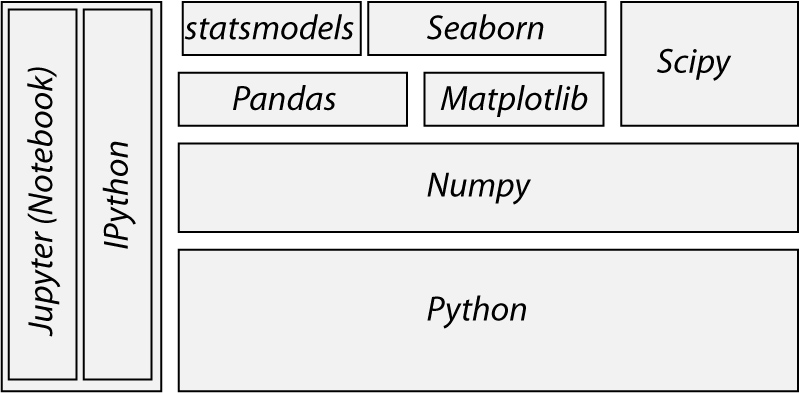
\includegraphics[width=0.5\textwidth]{../Images/ScientificPython.jpg}\\
  \caption{The structure of the most important Python packages for statistical applications.}
  \label{fig:scientificPython}
\end{figure}

For maximum flexibility, I started my session from the \emph{WinPython Command Prompt}, with the command \lstinline{ipython qtconsole}. The \emph{WinPython Command Prompt} is nothing else but a command terminal, with the environment variables set such that Python is readily found.

First IPython starts out telling you about the version of IPython and Python you are using, and listing the most important help calls.

\begin{figure}
  \centering
  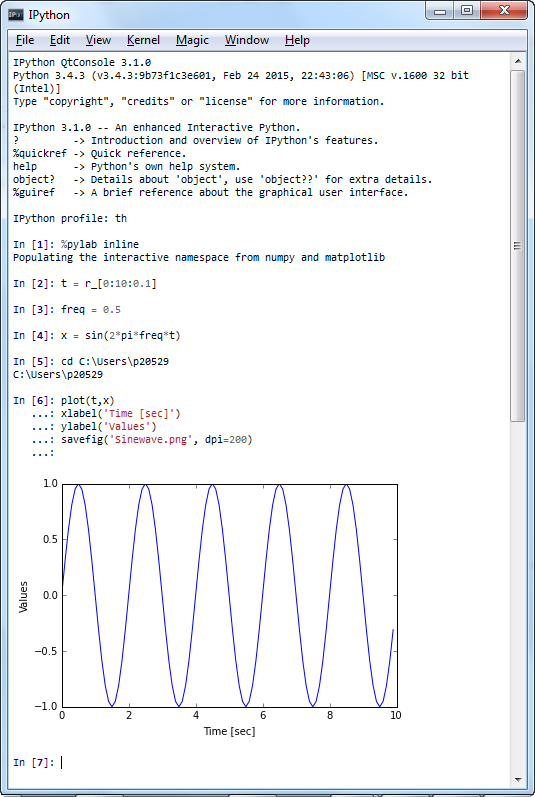
\includegraphics[width=0.85\textwidth]{../Images/qtConsole.png}\\
  \caption{Sample session in the IPython Qt-console.}
  \label{fig:qtConsole}
\end{figure}


\begin{itemize}
  \item \textbf{In [1]:} The first command \lstinline{%pylab inline} loads numpy and matplotlib into the current workspace, and directs matplotlib to show plots \emph{inline}. (This is automatically done if IPython is started with the commandline option "--pylab=inline".)

    To understand what is happening here requires a short detour into the structure of scientific Python. Fig.\ref{fig:scientificPython} shows the connection of the most important Python packages that are used in this book.

    \emph{Python} itself is an interpretative programming language, with no optimization for working with vectors or matrices or for producing plots. \emph{Packages} which extend the abilities of Python must be loaded explicitly. The most important package for scientific applications is \gls{numpy} \index{general}{numpy}, which makes working with vectors and matrices fast and efficient, and \emph{matplotlib}, which is the most common package used for producing graphical output. \Gls{scipy}\index{general}{scipy} contains important scientific algorithms. For the statistical data analysis, \lstinline{scipy.stats} contains the majority of the algorithms that will be used in this book. \emph{pandas} is a more recent addition, which has become widely adopted for statistical data analysis. It provides \emph{DataFrames}, which are labelled, 2-dimensional data structures, making work with data more intuitive and clearer. \emph{seaborn} extends the plotting abilities of \gls{matplotlib}, with a focus on statistical graphs. And \emph{statsmodels} contains many modules for statistical modeling, and for advanced statistical analysis. Both \emph{seaborn} and \emph{statsmodels} make use of the \emph{pandas'} DataFrames.

    \emph{IPython} provides the tools for interactive data analysis. It lets you quickly display graphs and change directories, explore the workspace, provides a command history etc. The ideas and base structure of IPython have been so successful that one component, the \emph{IPython Notebook} has been turned into a project of its own, \emph{Jupyter}, which is now also used by other languages like Julia, R, and Ruby.

  \item \textbf{In [2]:} The command \lstinline{t = r_[0:10:0.1]} is a shorthand version for \lstinline{t = arange(0, 10, 0.1)}, and generates a vector from 0 to 10, with a step size of 0.1.  \lstinline{_r} (and \lstinline{arange}) is a command in the numpy package. However, since \lstinline{numpy} has already been imported into the current workspace by IPython, we can use these commands right away.
  \item \textbf{In [4]:} Since \emph{t} is a vector, and \emph{sin} is a function from numpy, the sine-value is calculated automatically for each value of \emph{t}.
  \item \textbf{In [5]:} In Python scripts, changes of the current folder have to be performed with \lstinline{os.chdir()}. However, common task with interactive computing, like directory changes (\lstinline{%cd}), bookmarks for directories (\lstinline{%bookmark}), inspection of the workspace (\lstinline{%who} and \lstinline{%who}), etc, are implemented as \emph{IPython magic functions}.
  \item \textbf{In [6]:} Since we started out with the command \lstinline{%pylab inline}, IPython generates plots in the Qt-console, as shown in Fig. \ref{fig:qtConsole}. I have mentioned above that \emph{matplotlib} handles the graphics output. In the IPython Qt-console, you can switch between inline graphs and output into a separate graphics-window with \lstinline{%matplotlib inline} and \lstinline{%matplotlib qt4} (see Fig.\ref{fig:qt4}). This allows you to zoom in and pan, get the cursor position (which can be handy in helping to find outliers), and get interactive input with the command \lstinline{ginput}. matplotlib's plotting commands closely follow the MATLAB conventions. Note that also generating graphics files is very simple (here I generate the PNG-file "Sinewave.png", with a resolution of 200 dots-per-inch.)
\end{itemize}

\begin{figure}
  \centering
  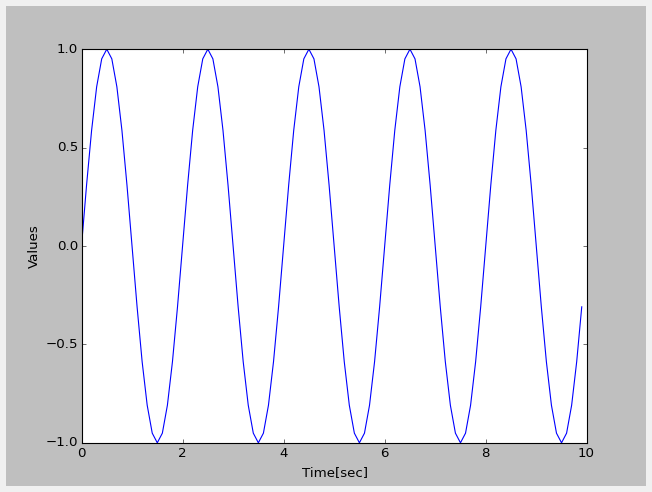
\includegraphics[width=0.65\textwidth]{../Images/qt4.png}\\
  \caption{Graphical output window, using the Qt4-framework. This allows you to pan, zoom, and get interactive input.}
  \label{fig:qt4}
\end{figure}


\subsection{Personalizing IPython}

When working on a new problem, I always start out with IPython. Once
I have the individual steps working, I use the IPython command \emph{\%history} to get the commands I have used, and switch to an integrated development environment (typically \emph{Wing} or \emph{Spyder}).

To start up IPython quickly in the location and with the configuration I like, I use the following tricks:

To personalize IPython, generate your own profile as shown below. Thereby, \emph{myname} has replaced with your login name, and \emph{mydir} with your home-directory (i.e. the directory that opens up when you run \lstinline{cmd} in Windows, or \lstinline{terminal} in Linux):

\subsubsection{In Windows}

\begin{itemize}
  \item Type Win+R, and start a command shell with \lstinline{cmd}
  \item In the newly created command shell, execute the following commands:
        \begin{lstlisting}
            ipython profile create myname
        \end{lstlisting}
        (This generates a folder $.ipython \backslash profile\_myname \backslash startup"$)
  \item Into this folder, place a file with e.g. the name $00\_myname.py$, containing
        \begin{lstlisting}
            import pandas as pd
            import os
            os.chdir(r'C:\mydir')
        \end{lstlisting}
        Note: since Windows uses "\" to separate directories, but "\" is also the escape character in strings, directory paths have to be preceded by "r", indicating \emph{raw strings}.
  \item Generate a file "ipy.bat" in \emph{mydir}, containing
      \begin{lstlisting}
      [Python-directory]\Scripts\ipython3 qtconsole --profile myname --pylab=inline
      \end{lstlisting}
\end{itemize}

To see all ipython notebooks for the course, do the following:
\begin{itemize}
    \item Type Win+R, and start a command shell with \lstinline{cmd}
    \item Run the commands
        \begin{lstlisting}
          cd [ipynb-directory]
          [Python-directory]\Scripts\ipython3 notebook --pylab=inline
        \end{lstlisting}
    \item Again, if you want, you can put this command sequence into a batch-file.
\end{itemize}


\subsubsection{In Linux}

\begin{itemize}
  \item Start a Linux terminal with the command \lstinline{terminal}

  \item In the newly created command shell, execute the following command
        \begin{lstlisting}
            ipython profile create myname
        \end{lstlisting}
        (This generates a folder $.ipython/profile\_myname/startup"$)
  \item Into this folder, place a file with e.g. the name $00\_myname.py$, containing
        \begin{lstlisting}
        import pandas as pd
        import os
        os.chdir(mydir)
        \end{lstlisting}
  \item In your .bashrc file, enter the line
      \begin{lstlisting}
          alias ipy='ipython3 qtconsole --profile myname --pylab=inline'
      \end{lstlisting}
  \item To see all IPython notebooks, do the following:
    \begin{itemize}
      \item Go to \emph{mydir}
      \item Create the file \emph{ipynb.sh}, containing the lines
        \begin{lstlisting}
            #!/bin/bash
            cd [wherever_you_have_the_ipynb_files]
            ipython3 notebook
        \end{lstlisting}
      \item Make the file executable, with \lstinline{chmod 755 ipynb.sh}
    \end{itemize}
\end{itemize}

Now you can start "your" ipython by just typing \lstinline{ipy}, and the notebooks by typing "ipynb.sh"

\subsubsection{In OSX}

Here the procedure should be the same as in Linux [CHECK!!!]

\subsection{Ipython Notebook}\index{general}{IPython!notebook}

Since approximately 2013 the \emph{IPython notebook} has become a very popular way to share research and results with the Python community. It allows to combine a structured layout, equation in the popular LaTex-format, and resulting graphs and videos.

\begin{figure}
  \centering
  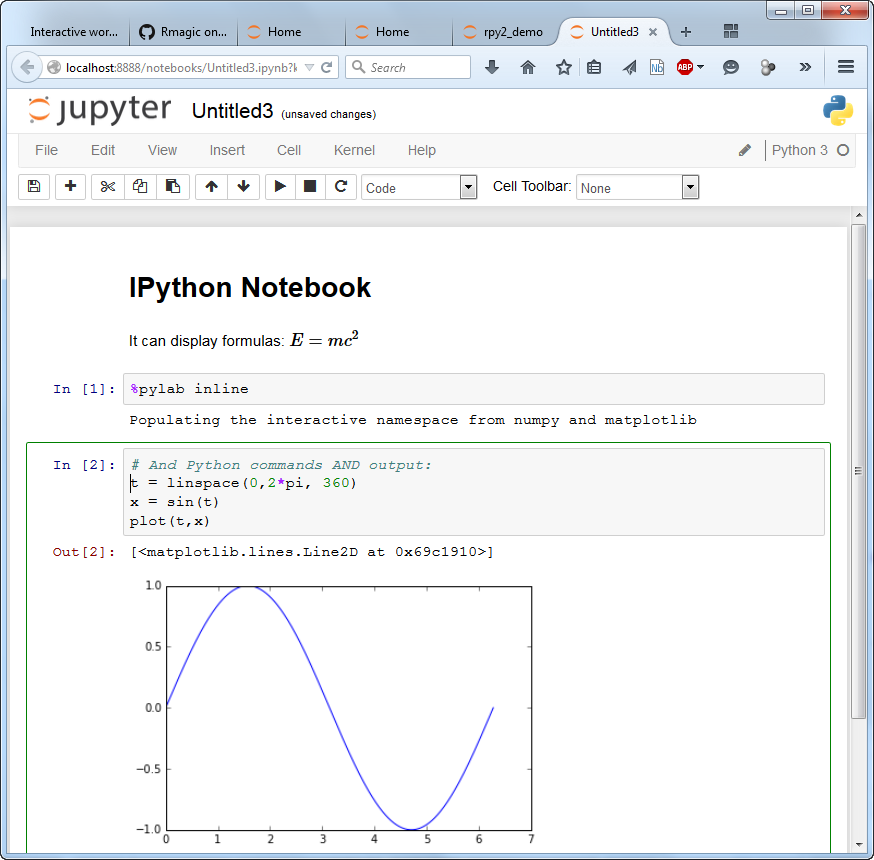
\includegraphics[width=0.85\textwidth]{../Images/ipython-notebook.png}\\
  \caption{The \emph{IPython Notebook} makes it easy to share research, formulas, and results.}
\end{figure}

\subsubsection{rpy2}\index{general}{rpy2}\index{general}{R (programming language)}

While Python is my preferred programming language, the world of advanced statistics is clearly dominated by \emph{R}. Like Python, R is completely free, and has a very active user community. While Python is a general programming language, R is optimized for the interactive work with statistical data. Many users swear that \emph{ggplot} provides the best-looking graphs for statistical data.

To combine the best of both worlds, the package \emph{rpy2} provides a way to transfer data from Python into R, execute commands in R, and transfer the results back into Python. In the IPython notebook, with rpy2 even R graphics can be fully utilized!

\begin{figure}
  \centering
  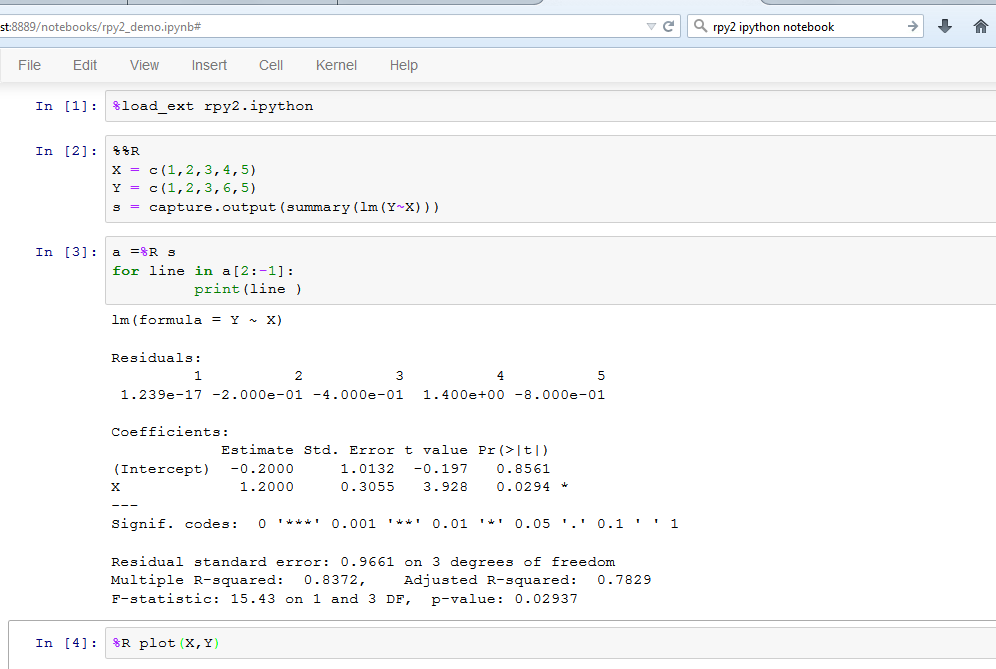
\includegraphics[width=0.85\textwidth]{../Images/ipython-rmagic.png}\\
  \caption{The output from R-commands is not working properly yet, and has been "hacked" here. However, this issue should be resolved soon.}
\end{figure}

\subsection{IPython Tips}

\begin{enumerate}
    \item Use IPython in the qtconsole, and start it in \emph{pylab}-mode: pylab: \texttt{ipython qtconsole ---pylab=inline}
    \item For help on e.g. \texttt{plot}, use \texttt{plot?} or \texttt{help(plot)}.
    \item Check out the help tips when you start ipython.
    \item Customize ipython on your computer, as described above: it will save you time in the long run!
    \item TAB-completion, for file- and directory names, variable names, AND for commands.
    \item To switch between inline and external graphs, use \; \texttt{\%matplotlib inline} and \; \texttt{\%matplotlib qt4}.
\end{enumerate}

\section{Developing Python Programs}

\subsection{First Python Script}

IPython is very helpful in working out the command syntax and sequence. The next step is to turn this in to a Python program that can be run from the command-line. This section introduces a fairly large number of Python conventions and syntax.

An efficient way to to turn IPython commands into a function is to

\begin{itemize}
  \item first obtain the command history with the command \lstinline{%hist}.
  \item copy the history into a good IDE (e.g. \emph{Wing}, see below)
  \item turn it into a working Python program by adding the relevant package information, etc.
\end{itemize}

In this case, this leads to

\lstinputlisting[label=py:pythonDemo,caption=pythonScript.py, language=Python, numbers=left]{../Code3/pythonScript.py}

The following modifications were made from the IPython history:

\begin{itemize}
  \item Files with the extension \emph{\.py} are called \emph{Modules}.
  \item \textbf{1-8:} It is comment to precede a Python module with a header block. Multiline comments are given between " ''' ". The first comment block describing the module should also contain information about author, date, and version number.
  \item \textbf{10:}  Single-line comments use " \# ".
  \item \textbf{11-13:} The required Python packages have to be imported explicitly. (In IPython, this is done by the command \lstinline{%pylab}.) It is customary to import \emph{numpy as np}, and \emph{matplotlib.pyplot}, the matplotlib module which contains all the plotting commands, as \emph{plt}.

  \item \textbf{16 etc:} The numpy command \emph{r\_} has to be addressed through the corresponding package name, i.e. \lstinline{np.r_}. (In IPython, \emph{\%pylab} took care of that.)
  \item \textbf{20:}  Note that also \emph{pi} is in numpy, so \lstinline{np.pi} is needed!
 \item \textbf{23 etc:}  All the plotting commands have to be preceded by their corresponding module, \emph{plt.}.
  \item \textbf{30:} Changes of the current directory require the \lstinline{os} package. In Windows, you have to deal with the additional problem that directories in path-names are separated by "", which is also used as the escape-character in strings. To take "" literally, a string has to be preceded by "r" (for "r"aw string).
  \item \textbf{34:} While IPython automatically shows graphical output, Python programs don't show the output until this is explicitly requested by \lstinline{plt.show()}. The idea behind this is to optimize the program speed, only showing the graphical output when it is all finished.
\end{itemize}

\begin{figure}
  \centering
  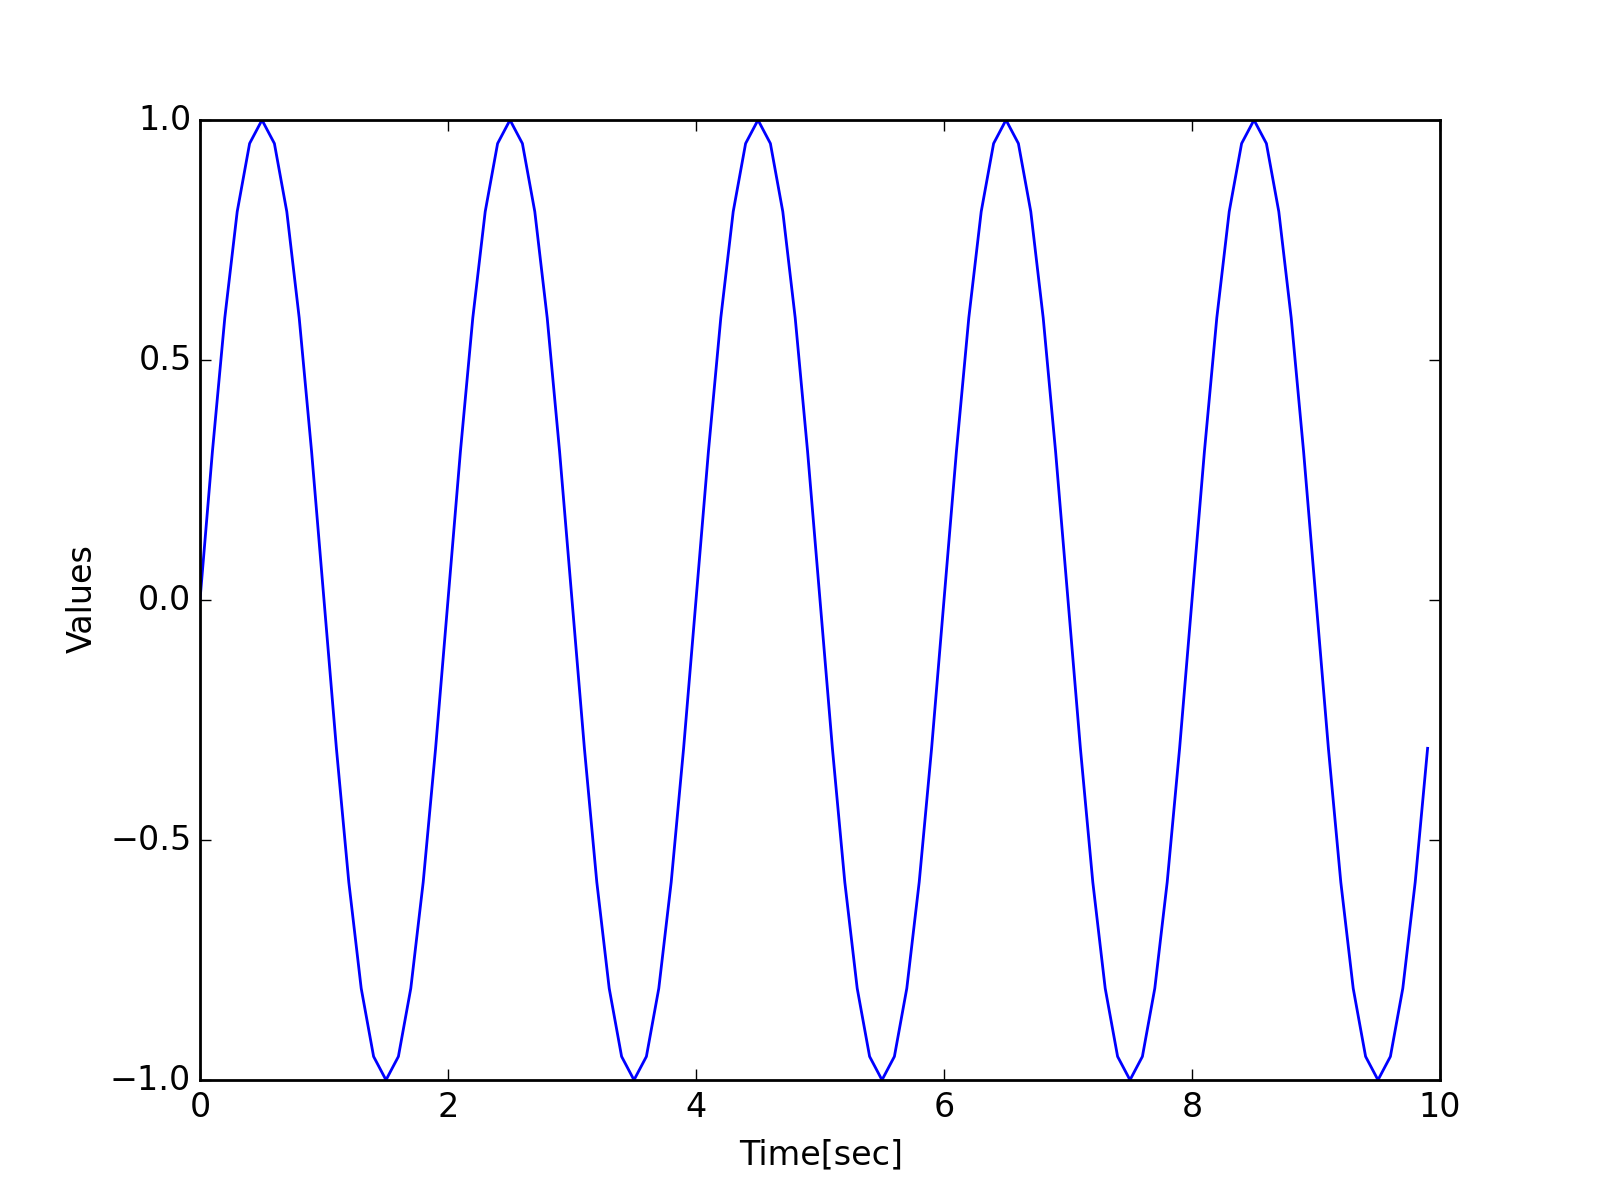
\includegraphics[width=0.5\textwidth]{../Images/Sinewave.png}\\
  \caption{Output file from "pythonScript.py".}
  \label{fig:pythonScript}
\end{figure}


\begin{figure}
  \centering
  \includegraphics[width=0.75\textwidth]{../Images/Wing.png}\\
  \caption{\emph{Wing}\index{general}{Wing} is my favorite development environment, with probably the best existing debugger for Python.}
\end{figure}

To write a program, I typically take the commands I have worked out in ipython with \lstinline{%history}, and take them to an IDE (integrated development environment): I either use \emph{Wing} (my clear favorite Python IDE, although it is commercial) or \emph{Spyder} (which is good and free). \emph{PyCharm} is another IDE with a good debugger, and has very good vim-emulation.

\begin{figure}
  \centering
  \includegraphics[width=0.75\textwidth]{../Images/spyder-screenshot.jpg}\\
  \caption{\emph{Spyder}\index{general}{Spyder} is a very good, free IDE.}
\end{figure}

\subsection{Functions, Modules, and Packages}

Python has different levels of modularization:

\begin{description}
  \item[Function] \Glspl{function} are defined by the keyword \lstinline{def}, and can be defined anywhere in Python. They return the object in the \lstinline{return} statement, typically at the end of the function.
  \item[Modules] \Glspl{module} is a file with the extension \emph{.py}. Modules can contain function definitions, as well as valid Python statements.
  \item[Packages] \Gls{package} is a folder containing multiple Python modules, and must have a file named \emph{\_\_init\_\_.py}. For example, \emph{numpy} is a Python package.
\end{description}

\subsubsection{Functions}
The following example shows how functions can be defined and used.

\lstinputlisting[label=py:pythonFunction,caption=pythonFunction.py, language=Python, numbers=left]{../Code3/pythonFunction.py}

\begin{itemize}
  \item \textbf{1-4:} Comment header.
  \item \textbf{6:} Since numpy will be required in that module, it has to be imported. To reduce the writing to a minimum, it is conventionally called \emph{np}.
  \item \textbf{8/9:} Function definition, and a comment describing the function. Note that the function block is defined by the indentation, not by any brackets of \emph{end} statements! This is a feature that irritates many Python novices, but that really helps to keep code clear and nicely formatted. Important: Python makes a difference between a tab and the equivalent amount of spaced. This can lead to errors which are really hard to detect, so you should use a good IDE that automatically converts tabs to spaces!
  \item \textbf{10:}
    \begin{itemize}
      \item The \lstinline{sum} command is taken from \emph{numpy}, so it has to be preceded by \lstinline{.np}.
      \item In Python, function arguments are indicated by round brackets (\emph{(...)}, whereas elements of lists, tuples, vectors, and arrays are indicated by square brackets (\emph{[...]}).
      \item In \emph{numpy} you can select elements of an array either with an in index (see line \textbf{19}), or with a boolean array as here (line \textbf{10}).
    \end{itemize}
  \item \textbf{13:} Python also uses round brackets to form groups of elements, so-called \emph{tuples}. And the \lstinline{return} statement does the obvious things: it returns elements from a function.
  \item \textbf{15:} Here quite a few new aspects of Python come together:
      \begin{itemize}
        \item Just like function definitions, \emph{if}-loops or \emph{for}-loops use indentation to define their context.
        \item Python conventionally uses underscores (\emph{\_-}) to indicate private variables, which are not used for typical programming tasks.
        \item Here we check the name \lstinline{\_\_name\_\_}, which is denoting the context of a module evaluation. If the module is run as a Python script, \lstinline{\_\_name\_\_} is set to \emph{\_\_main\_\_}. But if a module is imported, it is set to the name of the importing module. This way it is possible to add code to a function that is only used when the module is executed, but not when the functions in this module are \lstinline{import}ed by other modules (see below).
      \end{itemize}
  \item \textbf{16:} Definition of a \emph{numpy} array.
  \item \textbf{25:} When two elements are returned from a function \emph{(incomeAndExpenses}, they can be immediately assigned to two different Python objects (\emph{myIncome, myExpenses}.
  \item \textbf{26:} While there are different ways to produce formatted strings, this is probably the most elegant one: curly brackets (\emph{"{...}"}) indicate values that will be inserted, and can also contain formatting statements. The corresponding values are then passed into the string by the method \lstinline{format}.
\end{itemize}

\subsubsection{Modules}

To \emph{execute} a module from the commandline, type \lstinline{python pythonFunction.py}. In Windows, if the extension \emph{.py} is associated with the Python program, it suffices to double-click the module, or to type \lstinline{pythonFunction.py} on the commandline. In WinPython the association of the extension \emph{.py} with the Python function is set by the \emph{WinPython Control Panel.exe}, by the command \emph{"Register Distribution ..."} in the menu \emph{"Advanced"}.

To run a module in IPython, use the magic function \emph{\%run}:

\begin{lstlisting}
    In [56]: %run pythonFunction
    Your first transaction was a loss, and will be dropped.
    You have earned 23.00 EUR, and spent 10.00 EUR.
\end{lstlisting}

Note that you either have to be in the directory where the function is defined, or you have to give the full pathname.

If you import a module multiple times, Python recognizes that the module is already known, and skips later imports. If you want to override this, and explicitly want to re-import a module that has changed, you have to use the command \emph{reload} from the package \emph{importlib}:

\begin{lstlisting}
    from importlib import reload
    reload(pythonFunction)
\end{lstlisting}

The next example shows you how to import functions from one module into another one:

\lstinputlisting[label=py:pythonImport,caption=pythonImport.py, language=Python, numbers=left]{../Code3/pythonImport.py}

\begin{itemize}
  \item textbf{6:} Here the module \lstinline{pythonFunction} (that we have just discussed above) is imported. Note that the code in the section \lstinline{if \_\_name\_\_ == '\_\_main\_\_'} is NOT executed when the module is imported!
  \item textbf{12:} To access the function \emph{incomeAndExpenses} from the module \emph{pythonFunction}, I have to use \lstinline{incomeAndExpenses.pythonFunction(...)}
\end{itemize}

%  \item \textbf{14:} Function definitions can be made anywhere in the Python program. A peculiarity that is loved by many, but hated by many others, is the convention that the function definition is defined by the indentation, not by any explicit \emph{end} or by brackets. Just below the function definition (\textbf{15}) is the customary short function description. Not only functions, but also loops, if-statements etc. are defined by code indentation!
%  \item \textbf{17:} To group objects of the same type, Python uses \emph{lists}, which are indicated by square brackets (\emph{[...]}).
%  \item \textbf{18:} To address individual elements of a list, Python uses square brackets (\lstinline{pCoeff[0]}). Note that indexing starts at \emph{0}, not at \emph{1}! To square each element of the vector \lstinline{inData} is achieved by \lstinline{inData**2}.
%  \item \textbf{19:} The return value(s) of a function are indicated by \lstinline{return}. Since here we group elements of different types (a vector and a list), we don't use a \emph{Python tuple}, indicated by round brackets (\emph{(...)}). In contrast to lists, tuples are immutable.
%  \item \textbf{21:} This statement is related to the difference between \emph{importing} a module, and \emph{running} a module (see the last point in the \emph{IPython Tips} above.)
%       When the Python interpreter reads a source file, it executes all of the code found in it. Before executing the code, it will define a few special variables. For example, if the python interpreter is running that module (the source file) as the main program, it sets the special \lstinline{__name__} variable to have a value \lstinline{__main__}. If this file is being imported from another module, \lstinline{__name__} will be set to the module's name.

\subsection{Python Tips}

\begin{enumerate}
  \item Stick to the standard conventions.
      \begin{itemize}
        \item Every function should have documentation at the top.
        \item \texttt{import matplotlib.pyplot as plt}\\
            \texttt{import numpy as np}\\
            \texttt{import scipy as sp}\\
            \texttt{import pandas as pd}\\
            \texttt{import seaborn as sns}
      \end{itemize}
  \item To get the current directory, use \texttt{os.path.abspath(os.curdir)}.
  \item Everything in Python is an object: to find out about "obj", use \texttt{type(obj)} and \texttt{dir(obj)}.
  \item Learn to use the debugger.
  \item Know \emph{lists}, \emph{tuples}, and \emph{dictionaries}; also, know about \emph{numpy arrays} and \emph{pandas DataFrames}.
  \item Use functions a lot, and understand the \texttt{if \_\_name\_\_=='\_\_main\_\_':} construct.
  \item If you have all your personal functions in the directory \emph{mydir}, you can add this directory to your PYTHONPATH with the command
      \begin{lstlisting}
        import sys
        sys.path.append('mydir')
      \end{lstlisting}
\end{enumerate}

\section{Python Data Structures}

\begin{description}
  \item[Tuple ()] \index{general}{tuple}A collection of different things. Tuples are \emph{immutable}, i.e. they cannot be modified after creation.
  \item[List [] ] \index{general}{list}Lists are \emph{mutable}, i.e. their elements can be modified. Therefore lists are typically used to collect items of the same type (numbers, strings, ...).
  \item[Array [] ] \index{general}{array}Vectors\index{general}{vectors} and matrices, for numerical data manipulation. Defined in \emph{numpy}. Note that vectors and 1-d arrays are different: vectors \emph{cannot} be transposed!
  \item[Dictionary \{\}] \index{general}{dictionary}Dictionaries are unordered \emph{(key/value)} collections of content, where the content is addressed as \emph{dict['key']} (see example below).
  \item[DataFrame] \index{general}{dataframe}Data structure optimized for working with named, statistical data. Defined in \emph{pandas}. (See next chapter.)
\end{description}

\begin{lstlisting}
    In [1]: myTuple = ('abc', np.arange(0,3,0.2), 2.5)

    In [2]: myTuple[2]
    Out[2]: 2.5

    In [3]: myList = ['abc', 'def', 'ghij']

    In [4]: myList.append('klm')

    In [5]: myList2 = [1,2,3]

    In [6]: myList3 = [4,5,6]

    In [7]: myList2 + myList3
    Out[7]: [1, 2, 3, 4, 5, 6]

    In [8]: myArray = np.array(myList2)

    In [9]: myArray2 = np.array(myList3)

    In [10]: myArray + myArray2
    Out[10]: array([5, 7, 9])

    In [11]: myDict = dict(one=1, two=2, info='some information')

    In [12]: myDict2 = {'ten':1, 'twenty':20, 'info':'more information'}

    In [13]: myDict['info']
    Out[13]: 'some information'

    In [14]: myDict.keys()
    Out[14]: dict_keys(['one', 'info', 'two'])
\end{lstlisting}

\subsection{Indexing and Slicing}\index{general}{indexing}\index{general}{slicing}

For addressing individual elements in Python lists or tuples, or in numpy arrays, the following conventions are used (Fig. \ref{fig:indexing}):

\begin{figure}[H]
  \centering
  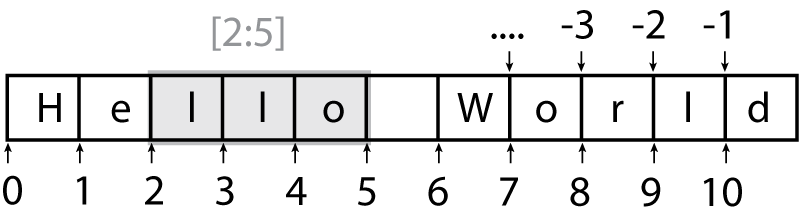
\includegraphics[width=0.75\textwidth]{../Images/IndexingAndSlicing.png}\\
  \caption{Conventions for Python Indexing and Slicing.}
  \label{fig:indexing}
\end{figure}

\begin{itemize}
  \item Indexing starts at 0, NOT at 1.
  \item The index refers to the \emph{pointer}, not to the variable.
  \item When one element is addressed, the element indicated by the pointer is selected. For example, with \lstinline{data = 'Hello World'}, \lstinline{data[1] gives the letter \emph{"e"}.
  \item Addressing a \emph{slice of data} (gray shaded area in Fig. \ref{fig:indexing}) returns the elements between the selected pointers.
        E.g. \lstinline{data[2:5]} returns \emph{"el"}. The number of elements returned (here \emph{3}) equals the difference between the selected pointers (here \emph{5-2}).
  \item When slicing, the third parameter indicates the step size. E.g. \lstinline{data[1::3]} produces \emph{"eood"}.
  \item You can also use negative indices, corresponding stepping backwards from the end of the object.
\end{itemize}

\subsubsection{Vectors and Arrays}

\emph{numpy} is the Python module that makes working with numbers efficient. By default, it produces vectors. The commands most frequently used to generate numbers are

\begin{description}
  \item[np.zeros] Generates zeros. Note that it takes only \emph{one} input. If you want to generate a matrix of zeroes, this input has to be a tuple containing the number of rows/columns!
  \item[np.ones] Generates ones.
  \item[np.random.randn] Generates normally distributed numbers, with a mean of 0 and a standard deviation of 1.
  \item[np.arange] Generates a range of numbers. Parameters can be \emph{start, end, steppingInterval}. Note that the end-value is \emph{excluded}!
  \item[np.linspace] Generates linearly spaced numbers.
  \item[np.array] Generates a numpy array from the given data.
\end{description}

\begin{lstlisting}
    import numpy as np

    np.zeros(3)
    >>>  array([ 0.,  0.,  0.])

    np.zeros( (2,3) )
    >>> array([[ 0.,  0.,  0.],
               [ 0.,  0.,  0.]])

    np.arange(3)
    >>> array([0, 1, 2])

    np.linspace(0,10,6)
    >>> array([  0.,   2.,   4.,   6.,   8.,  10.])

    np.arange(1,3,0.5)
    >>> array([ 1. ,  1.5,  2. ,  2.5])

    array([[1,2], [3,4]])
    >>> array([ [1, 2],
                [3, 4] ])
\end{lstlisting}

There are a few points that are peculiar to Python, and that are worth noting:

\begin{itemize}
  \item Matrices are simply \emph{lists of lists}. Therefore the first element of a matrix gives you the first row:
    \begin{lstlisting}
        import numpy as np
        Amat = np.array([ [1,2], [3,4] ])
        Amat[0]
        >>> array([1, 2])
    \end{lstlisting}
  \item A vector is not the same as a 1-dimensional matrix! This is one of the few un-intuitive features of Python, and can lead to mistakes that are hard to find. For example, vectors cannot be transposed, but matrices can.
      \begin{lstlisting}
        import numpy as np

        x = np.arange(3)
        Amat = np.array([ [1,2], [3,4] ])

        x.T == x
        >>> array([ True,  True,  True], dtype=bool)

        Amat.T == A
        >>> array([[ True, False],
                    [False,  True]], dtype=bool)
    \end{lstlisting}
\end{itemize}

\section{Plots in Python}

The Python core does not include any possibilities to generate plots. This is added by other packages. The by far most common package used for plotting is \Gls{matplotlib}\index{general}{matplotlib}. Matplotlib is not part of the core of Python. But if you installed Python with a scientific package like \emph{WinPython} or \emph{anaconda}, it will be included. Matplotlib is intended to mimic the style of Matlab. As such, users can either generate plots in the MATLAB style, or in the traditional Python style (see below).

Matplotlib contains a number of different modules and features:
\begin{description}
  \item[matplotlib.pyplot] This is the module that is commonly used to generate plots, and is by convention imported in Python functions and scripts with \lstinline{import matplotlib.pyplot as plt}. \emph{pyplot} \index{general}{pyplot} provides the interface to the plotting library in matplotlib. Pyplot handles a lot of little details, such as creating figures and axes for the plot, so that the user can concentrate on the data analysis.
  \item[matplotlib.mlab] Contains a number of functions that are commonly used in MATLAB, such as \lstinline{find}, \lstinline{griddata}, etc.
  \item["backends"] Matplotlib can produce output in many different formats, which are referred to as \emph{backends}\index{general}{backend}:
    \begin{itemize}
      \item In an \emph{Ipython Notebook}, or in an \emph{IPython Qt-console}, the command \lstinline{%matplotlib inline} directs output into the current browser window. (\lstinline{%pylab inline} is a combination of loading pylab, and directing plot-output inline.
      \item In the same environment, \lstinline{%matplotlib qt4} directs the output into a separate graphics window (Fig. \ref{fig:qt4}). This allows panning and zooming the plot, and interactive selection of points on the plot by the user.
      \item In addition, output can be directed to external files, e.g. in PDF, PNG, or JPG format.
    \end{itemize}
\end{description}

\emph{pylab}\index{general}{pylab} is a convenience module that bulk imports matplotlib.pyplot (for plotting) and numpy (for mathematics and working with arrays) in a single name space. Although many examples use pylab, it is no longer recommended, and should only be used in IPython, to facilitate interactive development of code.

\subsection{Interactive plots}

Matplotlib provided different ways how to interact with the user. Unfortunatly, this interaction is less intuitive than in Matlab. To bypass most of these problems, you can base your code on the examples below:

\PyImg "interactivePlots.py" (p \pageref{py:interactivePlots}) gives a short demonstration of Python for scientific data analysis.
\index{python}{interactivePlots}

\subsection{Graphical Output in Python: Functional and Object-oriented Approach}

Python plots can be generated in a MATLAB-like style, or in an object oriented, more pythonic way. These styles are all perfectly valid, and each have their pros and cons. The only caveat is to avoid mixing the coding styles for your own code.

First, consider the frequently used pyplot style:

\begin{lstlisting}
    # Import the required packages, with their conventional names
    import matplotlib.pyplot as plt
    import numpy as np

    # Generate the plot
    x = np.arange(0, 10, 0.2)
    y = np.sin(x)
    plt.plot(x, y)

    # Display it on the screen
    plt.show()
\end{lstlisting}

Note that the creation of the required figure and an axes is done automatically by pyplot.

Second, a more pythonic, object oriented style, which may be clearer when working with multiple figures and axes:

\begin{lstlisting}
    # Import the required packages
    import matplotlib.pyplot as plt
    import numpy as np

    # Generate the data
    x = np.arange(0, 10, 0.2)
    y = np.sin(x)

    # Generate the (first) plot
    fig = plt.figure()

    # On that plot, add one axis
    ax = fig.add_subplot(111)

    # On that axis, plot the x/y-data
    ax.plot(x, y)

    # Display the resulting plot
    plt.show()
\end{lstlisting}

Next, the same example using a pure MATLAB-style:

\begin{lstlisting}
    from pylab import *
    x = arange(0, 10, 0.2)
    y = sin(x)
    plot(x, y)
\end{lstlisting}

So, why all the extra typing as one moves away from the pure MATLAB-style? For very simple things like this example, the only advantage is academic: the wordier styles are more explicit, more clear as to where things come from and what is going on. For more complicated applications, this explicitness and clarity becomes increasingly valuable, and the richer and more complete object-oriented interface will likely make the program easier to write and maintain.

Here an example, to get you started with Python. For interactive work, it is
simplest to use the \emph{pylab mode}, as shown in the example below.

\subsubsection{Example-Session}

\PyImg "gettingStarted.py" (p \pageref{py:gettingStarted_ipy}) gives a short demonstration of Python for scientific data analysis.
\index{python}{gettingStarted}


\section{Pandas}\index{general}{Pandas}

\href{http://pandas.pydata.org/.}{pandas} is a widely used Python package which has been contributed by Wes McKinney. It provides data structures suitable for statistical analysis, and adds functions that facilitate
data input, data organization, and data manipulation. It is common to \lstinline{import pandas as pd}, which reduces the typing a bit.

A good introduction to pandas can be found under
\url{http://www.randalolson.com/2012/08/06/statistical-analysis-made-easy-in-python/}

\subsection{Data Handling}


To handle labeled data, pandas introduces \emph{DataFrame} objects. A DataFrame is a 2-dimensional labeled data structure with columns of potentially different types. You can think of it like a spreadsheet or SQL table. It is generally the most commonly used pandas object.
At first, handling data with Pandas feels a bit unusual. To get you started, let me give you a specific example:

\begin{lstlisting}
    import numpy as np
    import pandas as pd

    t = np.arange(0,10,0.1)
    x = np.sin(t)
    y = np.cos(t)

    df = pd.DataFrame({'Time':t, 'x':x, 'y':y})
\end{lstlisting}

In Pandas, rows are addressed through "indices", and columns through their "column" name.
To address the first column only, you have two options:

\begin{lstlisting}
    df.Time
    df['Time']
\end{lstlisting}

If you want to extract two columns at the same time, ask for several variables in a list:

\begin{lstlisting}
    data = df[['Time', 'y']]
\end{lstlisting}

To display the first or last rows, use

\begin{lstlisting}
    data.head()
    data.tail()
\end{lstlisting}

For e.g. rows 5-10 (note that there are 6 numbers), use

\begin{lstlisting}
    data[4:10]
\end{lstlisting}

as $10-4=6$. (I know, the array indexing takes some time to get used to. Just keep in mind that Python addresses the \emph{locations between} entries, not the entries, and that it starts at $0$!!).

To extract rows and columns in one go, use

\begin{lstlisting}
    df[['Time', 'y']][4:10]
\end{lstlisting}

You can also apply the standard row/column notation, by using the method "ix":

\begin{lstlisting}
    df.iloc[[0,2],4:10]
\end{lstlisting}

Finally, sometimes you want to have direct access to the data, not to the DataFrame. You can do this with

\begin{lstlisting}
    data.values
\end{lstlisting}

\subsubsection{Note: Data selection}

While pandas' DataFrames are similar to numpy arrays, their philosophy is different, and I have wasted a lot of nerves addressing data correctly. Therefore I want to explicitly point out the differences here:

\begin{description}
  \item[numpy] handels \emph{rows} first. E.g. data[0] is the first row of an array
  \item[pandas] starts with the columns. E.g. df['values'][0] is the first element of the column 'values'.
\end{description}

If a DataFrame has labelled rows, you can extract for example the row "rowlabel" with with \lstinline{df.loc['rowlabel']}. If you want to address a row by its number, e.g. row number "15", use \lstinline{df.iloc[15]}. You can also use \emph{iloc} to address \emph{rows/columns}, e.g. \lstinline{df.iloc[2:4,3]}.

Slicing of rows also works, e.g. \lstinline{df[0:5]} for the first 5 rows. A sometimes confusing convention is that if you want to slice out a single row, e.g. row "5", you have to use \lstinline{df[5:6]}. If you use \lstinline{df[5]} alone, you get an error!

\subsection{Grouping}

Pandas offers powerful functions to handle missing data and "nans". It also allows more complex types of data manipulation like pivoting.
For example, you can use data-frames to efficiently group objects, and do a statistical evaluation of each group. The following data are simulated (but realistic) data of a survey on how many hours a day people watch on the TV, grouped into "m"ale and "f"emale responses:

\begin{lstlisting}
    data = pd.DataFrame({
        'Gender': ['f', 'f', 'm', 'f', 'm', 'm', 'f', 'm', 'f', 'm'],
        'TV': [3.4, 3.5, 2.6, 4.7, 4.1, 4.0, 5.1, 4.0, 3.7, 2.1]
        })

    #--------------------------------------------
    # Group the data
    grouped = data.groupby('Gender')

    # Do some overview statistics
    print(grouped.describe())

    # Plot the data:
    grouped.boxplot()

    #--------------------------------------------
    # Get the groups as DataFrames
    df_female = grouped.get_group('f')

    # Get the corresponding numpy-array
    values_female = grouped.get_group('f').values

    # or equivalently
    groups = grouped.groups
    values_female = groups['f']

\end{lstlisting}

produces

\begin{lstlisting}
                        TV
    Gender
    f      count  5.000000
           mean   4.080000
           std    0.769415
           min    3.400000
           25%    3.500000
           50%    3.700000
           75%    4.700000
           max    5.100000
    m      count  5.000000
           mean   3.360000
           std    0.939681
           min    2.100000
           25%    2.600000
           50%    4.000000
           75%    4.000000
           max    4.100000
\end{lstlisting}

\begin{figure}[H]
  \centering
  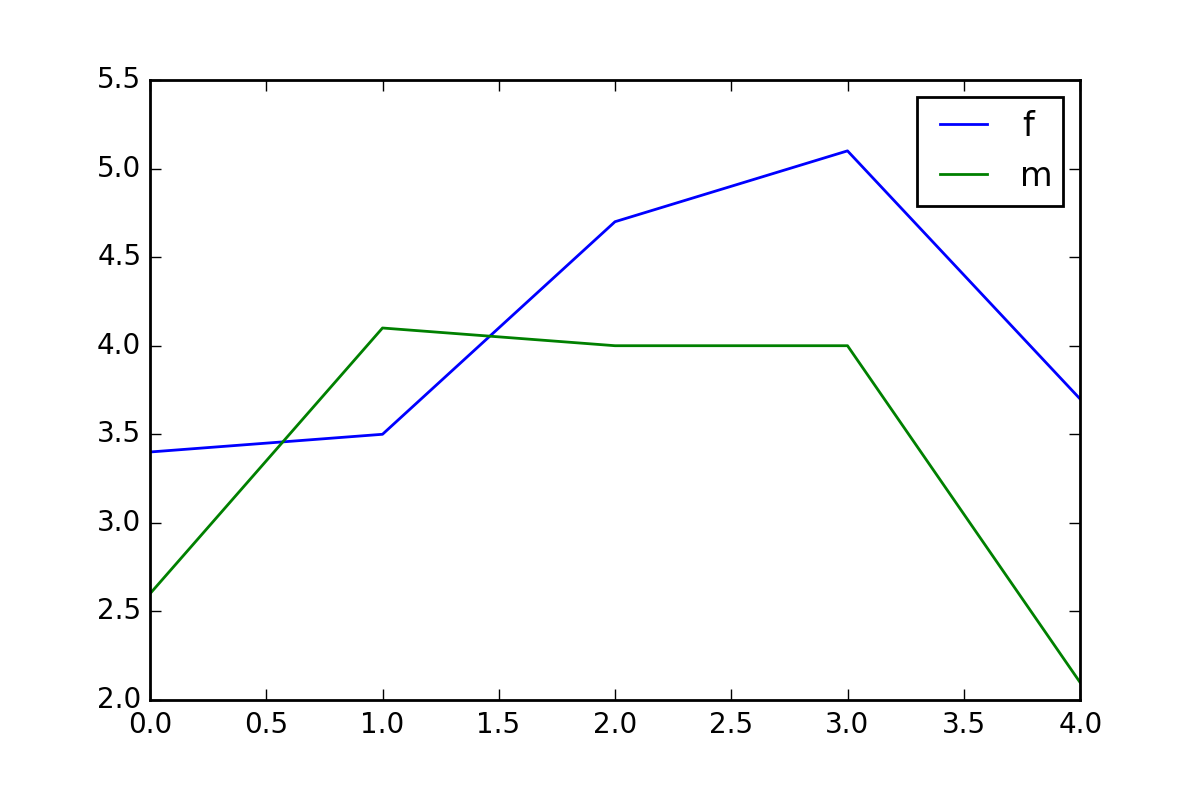
\includegraphics[width=0.75\textwidth]{../Images/grouped.png}\\
\end{figure}

For statistical analysis, pandas becomes really powerful if you combine it with \emph{statsmodels} (see below).

\section{Statsmodels}\index{general}{statsmodels}

\href{http://statsmodels.sourceforge.net/.}{statsmodels} is a Python package contributed to the community by the statsmodels development team. It has a very active user community, and has in the last five years massively improved the suitability of Python for statistical data analysis. \emph{statsmodels} provides classes and functions for the estimation of many different statistical models, as well as for conducting statistical tests, and statistical data exploration. An extensive list of result statistics are available for each estimator. \emph{statsmodels} also allows the formulation of models with the popular formula language based on the notation introduced by Wilkinson and Rogsers (\cite{Wilkinson1973}, and also used by $S$ and $R$, the leading statistics package. For example, data on the connection between academic "success", "intelligence" and "diligence" can be described with the model

\begin{equation*}
    success \sim intelligence * diligence
\end{equation*}

 which would capture the direct effect of "intelligence" and "diligence", as well as the interaction. You find more information on that topic in the section "Statistical Models".

While for complex statistical models R still has an edge, python has a much clearer and more readable syntax, and is arguably more powerful for the data manipulation often required for statistical analysis.

\PyImg "statsmodelsIntro.py" (p \pageref{py:statsmodelsIntro}) shows you how the combination of pandas and statsmodels can be used for data analysis.
\index{python}{statsmodelsIntro}

\section{Seaborn}\index{general}{seaborn}

\href{http://statsmodels.sourceforge.net/.}{seaborn} is a Python visualization library based on Matplotlib. Its primary goal is to provide a concise, high-level interface for drawing statistical graphics that are both informative and attractive.

\begin{lstlisting}
        x = linspace(1, 7, 50)
        y = 3 + 2*x + 1.5*randn(len(x))
        sns.regplot(x,y)
\end{lstlisting}

already produces a nice and informative regression plot (Fig. \ref{fig:seaborn}).

\begin{figure}[ht]
  \centering
  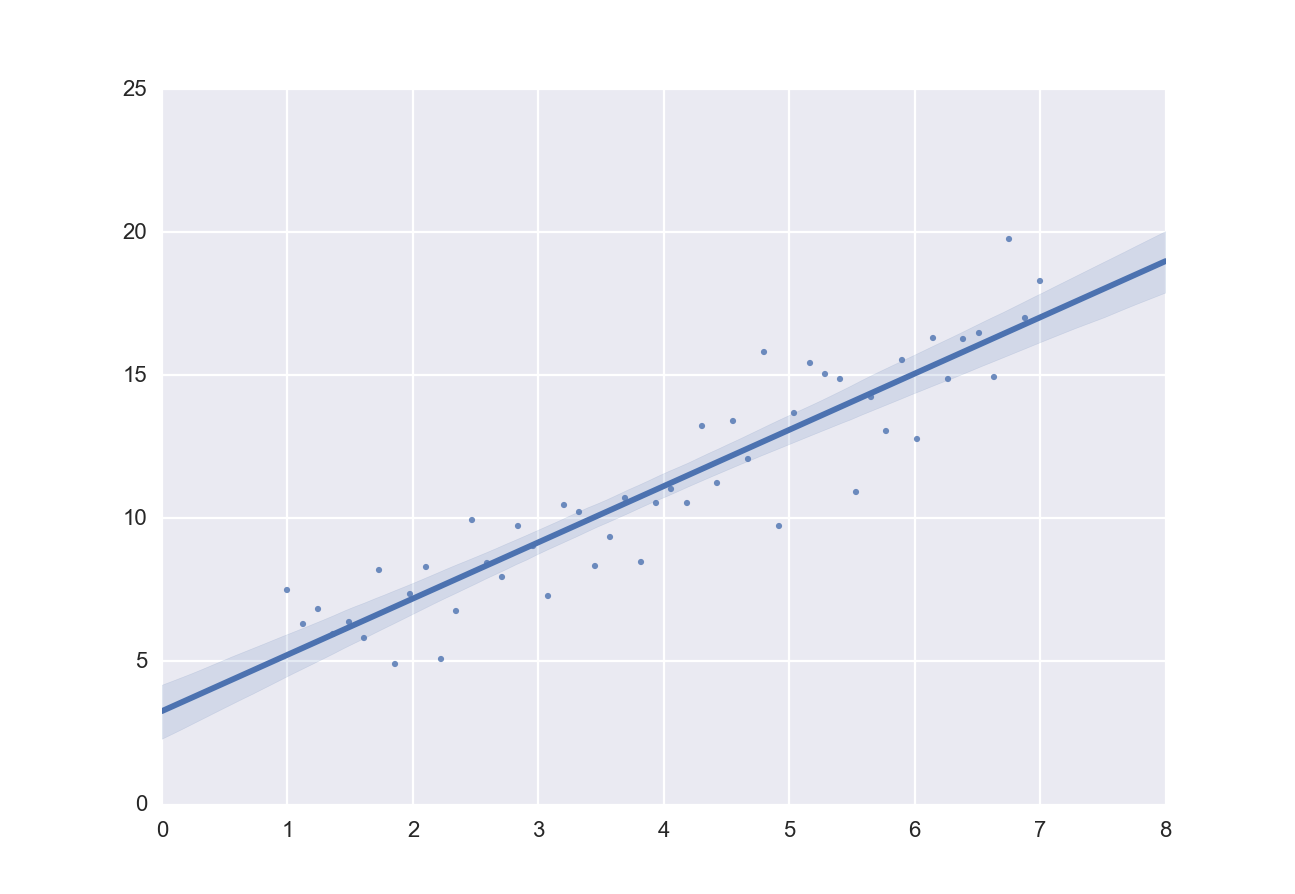
\includegraphics[width=0.5\textwidth]{../Images/regplot.png}\\
  \caption{Regression plot, from \emph{seaborn}. The main axis shows the data, the best-fit line, and the confidence intervals for the fit. It also provides the Pearson Correlation Coefficient, and the p-value for the inclination. The additional axes on top and on the right show histogram and Kernel-Density-Plots for the x- and y-data, respectively.}
  \label{fig:seaborn}
\end{figure}

\subsection{General Routines}
Here is also a good place to introduce the short function that we will use a number of times to simplify the reading in of data:

\PyImg "getData.py" (p \pageref{py:getData}) Gets the input data for many Python programs in this script.
\index{python}{getData}

\section{Exercises}

\begin{itemize}
  \item Read in data from different sources:
  \begin{itemize}
    \item A CVS-file with a header ('Data\textbackslash data\_kaplan\textbackslash swim100m.csv')
    \item An MS-Excel file ('Data\textbackslash data\_others\textbackslash GLM\_data\textbackslash Table 6.6 Plant experiment.xls')
    \item Data from the WWW (see "readZip.py" \ref{py:readZip})
  \end{itemize}
  \item
  \begin{itemize}
      \item Generate a pandas dataframe, with the x-column time stamps from 0 to 10 sec, at a rate of 10 Hz, the y-column data values with a sine with 1.5 Hz, and the z-column the corresponding cosine values. Label the x-column "Xvals", and the y-column "YVals", and the z-column "ZVals".
      \item Show the head of this dataframe
      \item Extract the data in lines 10-15 from "Yvals" and "ZVals", and write them to the file "out.txt".
  \end{itemize}
\end{itemize}
